\documentclass[DIV=14, a4paper, 12pt, headsepline, numbers=noenddot, bibliography=totoc, index=totoc, version=first, twoside, BCOR=2cm]{scrbook}
      
\usepackage[slantedGreek]{mathptmx}

% usage of zapf chancery as calligraphic font instead of rsfs
\DeclareSymbolFont{symbols}%
  {OMS}{pzc}{m}{n}
\DeclareSymbolFontAlphabet{\mathcal}%
  {symbols}
  
\usepackage{scrhack}
\usepackage{graphicx}
\usepackage{amsmath,amsfonts,amssymb}
\usepackage[utf8]{inputenc}
\usepackage{booktabs}
\usepackage{float}
%\heavyrulewidth=0.1em
\usepackage{makeidx}
\usepackage[german,english]{babel}
\usepackage{ifthen}
\usepackage{color}

\renewcommand{\topfraction}{1.0}    % Bilder duerfen auch direkt am
                                    % Seitenanfang sein
\renewcommand{\bottomfraction}{1.0} % Bilder duerfen auch direkt am
                                    % Seitenende sein

\newcommand{\remark}{\tiny \normalsize}
\newcommand{\trademark}{\tiny\texttrademark \normalsize}

%%%%%%%%%%%%%%%%%%%%%%%%%%%%%%%%%%%%%%%%%%%%%%%%%%%%%%%%%%%%%%%%%%%%%%%%%%%%%%
%% NEWCOMMAND \datetitle
%%
%% \datetitle{Title}{Author}{Matrikennummer}{Betreuer}
%%%%%%%%%%%%%%%%%%%%%%%%%%%%%%%%%%%%%%%%%%%%%%%%%%%%%%%%%%%%%%%%%%%%%%%%%%%%%%
\newcommand{\codesigntitle}[5]
{ \begin{titlepage}

  \titlehead
  { \hspace*{-18mm}
    \parbox[t]{14.4cm}{
        \parbox{76mm}{
        \vspace*{-25mm}
        
\includegraphics[width=35mm]{bilder/codesign}
      }
      \hfill
      \parbox{35mm}{
        \vspace*{-23mm}
        
\includegraphics[width=76mm]{bilder/FAU_Logo}
      }
    }
  }
  \title{{\parbox{0mm}{}\\[1cm]\huge \sffamily \bfseries{#1}}\\[4mm] \Huge{#2}}

  \ifthenelse{\boolean{englishDocument}}
  { \author{\Large by\\[4mm]
    \Large {\textbf #3}\\[2mm]
    \large Matrikel-Nr.: #4\\[7mm]
    \Large Supervision:\\ #5\\[16mm]}
    \date{\dateenglish{\today}}
  }
  { \author{\Large von\\[4mm]
    \Large {\textbf #3}\\[2mm]
    \large Matrikel-Nr.: #4\\[7mm]
    \Large Betreuung:\\ #5\\[16mm]}
    \date{\dategerman{\today}}
  }
  \thispagestyle{empty}
  \ifthenelse{\boolean{englishDocument}}
  { \lowertitleback{This document was produced with the typesetting system \LaTeX2e.}
  }
  { \lowertitleback{Dieses Dokument wurde mit dem Textsatzsystem \LaTeX2e erstellt.}
  }
  
  \end{titlepage}   

  \maketitle
}

\newboolean{printVersion}
\setboolean{printVersion}{true}      % default setting
\newboolean{englishDocument}
\setboolean{englishDocument}{false}  % default setting


\usepackage{etoolbox}
\makeatletter
\patchcmd{\scr@startchapter}{\if@openright\cleardoublepage\else\clearpage\fi}{}{}{}
\makeatother

\makeindex


%
% if printVersion == true  => no hyperlinks are generated
%                 == false => colored hyperlinks are generated
%
\setboolean{printVersion}{false}

%
% if englishDocument == true  => BABEL english and english dates are used
%                    == false => BABEL german and german dates are used
%
\setboolean{englishDocument}{false}

\newcommand{\studname}{Bastian Kauschke}

\ifthenelse{\boolean{printVersion}}{}{\usepackage[colorlinks=false]{hyperref}}
\usepackage{cite}


\begin{document}
\ifthenelse{\boolean{englishDocument}}
{ \selectlanguage{english}
}
{ \selectlanguage{german}
}

\frontmatter

\codesigntitle{Seminararbeit}{Backtracking}{\studname}{22442706}{Prof. Oliver Keszöcze}

\mainmatter
\chapter*{Zusammenfassung}

Viele Probleme der Informatik, zum Beispiel Wegsuche, Schachengines und 
das Ausführen logischer Programme \cite[p. ~19]{DBLP:journals/jlp/SomogyiHC96}, lassen sich durch Backtracking, auch Tiefensuche genannt, lösen.
Basierend auf Donald Knuths "`The Art of Computer Programming"'\cite{TAOCP} wird im folgenden diese Vorgehensweise 
vorgestellt und für einige Probleme Lösunsansätze implementiert. Alle hier verwendeten Programmschnipsel wurden in \textbf{Rust} implementiert und sind
dokumentiert auf \textbf{github}\cite{Kauschke} neben einigen Benchmarks zu finden.

\chapter{Einleitung}\label{einleitung}
Es ist oft möglich, Probleme als eine Sequenz $x_{1}, x_{2}, x_{3} \dots x_{n}$, für 
welche die Bedingung $P_{n}(x_{1}, x_{2}, x_{3} \dots x_{n})$ gelten soll, darzustellen.
Damit Backtracking zu deren Lösung eingesetzt werden kann, müssen außerdem noch
Untereigenschaften $P_{v}(x_{1}, x_{2}, x_{3} \dots x_{v})$ für alle $v \in [ \, 0, n) \,$ 
mit folgenden Eigenschaften existieren:
\begin{enumerate}
  \item $P_{0}()$ gilt immer
  \item $P_{v + 1}(x_{1}, x_{2}, x_{3} \dots x_{v + 1})$ gilt nur, wenn $P_{v}(x_{1}, x_{2}, x_{3} \dots x_{v})$ gilt
  \item wenn $P_{v}(x_{1}, x_{2}, x_{3} \dots x_{v})$ gilt, ist $P_{v + 1}(x_{1}, x_{2}, x_{3} \dots x_{v+1})$ einfach zu testen
\end{enumerate}

Somit kann man alle Sequenzen $x_{1}, x_{2}, x_{3} \dots x_{v} \dots x_{q}$ mit $q > v$ ignorieren,
falls $P_{v}(x_{1}, x_{2}, x_{3} \dots x_{v})$ nicht gilt.
Der darauf basierende Backtracking Algorithmus \textbf{B} kann nun wie folgt implementiert werden:
\begin{minted}[linenos, fontsize=\small]{rust}
pub fn b<T: Sequence>(initial: T, n: usize) -> Vec<T> {
    if !initial.satisfies_condition() {
        return Vec::new();
    } else if n == 0 {
        return vec![initial];
    }

    // all sequences of length n which satisfy the condition
    let mut results = Vec::new();

    // the current sequence, starts with just the initial state
    let mut states = Vec::new();

    let steps = initial.next_steps().into_iter();
    states.push((initial, steps));

    // run while there is still a state with an unchecked next step
    while let Some((state, steps)) = states.last_mut() {
        // take the next unchecked possible step of the current state,
        // in case there are no unchecked steps left,
        // simply discard the current state as all possible
        // sequences have already been tried.
        if let Some(step) = steps.next() {
            // compute the result of this step
            let next_state = state.apply_step(step);
            // does this new state still satisfy the condition,
            // if not we can simply discard it
            if next_state.satisfies_condition() {
                // if the sequence is already n elements long,
                // it is correct and can be added to results.
                // Otherwise we push it onto the stack.
                if states.len() < n {
                    let next_steps = next_state.next_steps().into_iter();
                    states.push((next_state, next_steps));
                } else {
                    results.push(next_state);
                }
            }
        } else {
            states.pop();
        }
    }

    results
}
\end{minted}

Um ein Problem mit diesem Algorithmus lösen zu können, benötigt man einen Datentyp, welcher den momentanen Zustand
der Sequenz speichern kann und das folgende Interface implementiert:
\begin{minted}[linenos, fontsize=\small]{rust}
/// A required set of methods needed for the generic backtracking algorithms.
pub trait Sequence {
    type Step;
    type Steps: IntoIterator<Item = Self::Step>;

    /// Checks if this sequence satisfies its condition.
    ///
    /// This function can assume that the  parent of `self` satisfied this condition.
    fn satisfies_condition(&self) -> bool;

    /// generates all possible next steps at this current state.
    fn next_steps(&self) -> Self::Steps;

    /// applies a `step` to `self`, returning the resulting sequence.
    ///
    /// this function will only be called if `self.satisfies_condition() == true`.
    fn apply_step(&self, step: Self::Step) -> Self;
}
\end{minted}
\chapter{Queens}
Eines der bekanntesten Anwendungsmöglichkeiten für Backtracking ist das n-Damen Problem.
Gesucht wird die Anzahl der Möglichkeiten $n$ Damen auf einem $n * n$ Schachbrett aufzustellen, sodass
keine Dame von einer anderen bedroht wird. Dies ist gegeben, wenn jede Zeile, Spalte und Diagonale jeweils von nur einer Dame
besetzt wird. Abbildung \ref{fig:n4} zeigt sowohl eine korrekte als auch eine inkorrekte Lösung für das Problem.
\begin{figure}
  \centering
  \begin{subfigure}{0.4\linewidth}
    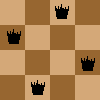
\includegraphics[width=\linewidth]{queensRight.png}
    \caption{Richtig}
  \end{subfigure}
  \begin{subfigure}{0.4\linewidth}
    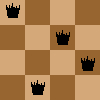
\includegraphics[width=\linewidth]{queensWrong.png}
    \caption{Falsch}
  \end{subfigure}
  \caption{n-Damen Problem}
  \label{fig:n4}
\end{figure}

\section{Implementierung}
Es dürfen keine 2 Damen in der selben Reihe sein. Eine mögliche Implementierung ist somit ein Liste, in welcher der Eintrag
$n$ die Position der Dame in der $n$-ten Reihe representiert. Der Initialzustand beim Backtracking ist ein leeres Schachbrett.
\begin{minted}[fontsize=\small, linenos]{rust}
pub struct Queens {
    /// dimension of the chessboard
    n: usize,
    /// currently occupied rows
    rows: Vec<usize>,
}
  
impl Queens {
    /// creates a new empty chess board of size `n`
    pub fn new(n: usize) -> Self {
        Self {
            n,
            rows: Vec::new(),
        }
    }
}
\end{minted}
Um diese Struktur nun in Algorithmus \textbf{B} zu verwenden, muss noch \mintinline{rust}{trait Sequence} implementiert werden:
\begin{minted}[fontsize=\small, linenos]{rust}
impl Sequence for Queens {
    type Step = usize;
    type Steps = Range<Self::Step>;

    /// checks if the most recently placed queen was placed on a free tile
    fn satisfies_condition(&self) -> bool {
        if self.rows.is_empty() {
            return true;
        }

        // the row of the last queen
        let k = self.rows.len() - 1;

        // for all previous queens
        for j in 0..self.rows.len() - 1 {
            let k_col = self.rows[k] as isize;
            let j_col = self.rows[j] as isize;

            // check if the queen at row `j` shares a column or diagonal
            // with the queen at row `k`
            if k_col == j_col || (j_col - k_col).abs() as usize == k - j {
                return false;
            }
        }
        true
    }

    /// returns all possible columns
    fn next_steps(&self) -> Self::Steps {
        0..self.n
    }

    /// clones `self` and adds the queen at `column` at the next free row
    fn apply_step(&self, column: Self::Step) -> Self {
        let mut rows = self.rows.clone();
        rows.push(column);
        Self { n: self.n, rows }
    }
}
\end{minted}
Nun kann man Algorithmus \textbf{B} zum Lösen des $n$-Damen Problems verwenden:
\begin{minted}{rust}
let results = b(Queens::new(4), 4);
\end{minted}
\section{B*}
Es gibt noch viele Möglichkeiten diese Lösung zu optimieren. Knuth verwendet einige davon im Algorithmus \textbf{B*}\cite[p. 4]{TAOCP}.
\subsection{Bitsets}
Die bisherige Lösung muss bei jeder neuen Dame alle vorherigen Damen einzeln überprüfen. Eine 
andere Option ist für jede Spalte und Diagonale zu speichern, ob sie momentan besetzt ist.
Man benötigt so etwas mehr Speicherplatz, reduziert aber die Anzahl der Speicherzugriffe gewaltig. 
Das kann durch 3 Bitsets mit der Verteilung aus Abbildung \ref{bitsets} implementiert werden.
\begin{figure}
  \centering
  \begin{subfigure}{0.3\linewidth}
    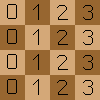
\includegraphics[width=\linewidth]{../img/columns.png}
    \caption{Spalten}
  \end{subfigure}
  \begin{subfigure}{0.3\linewidth}
    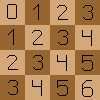
\includegraphics[width=\linewidth]{../img/left_diagonals.png}
    \caption{Gegendiagonale}
  \end{subfigure}
  \begin{subfigure}{0.3\linewidth}
    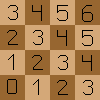
\includegraphics[width=\linewidth]{../img/right_diagonals.png}
    \caption{Hauptdiagonale}
  \end{subfigure}
  \caption{Bitsets}
  \label{bitsets}
\end{figure}

\subsection{Speicherwiederverwendung}
Da \mintinline{rust}{trait Sequence} bei jedem Schritt eine neues Object benötigt, kann das
Schachbrett nicht wiederverwendet werden. Indem man die zuletzt verwendete Dame beim Backtracking
wieder entfernt, wird insgesamt nur ein Array benötigt.

\subsection{Implementierung}
\begin{minted}[fontsize=\small, linenos]{rust}
pub fn b_star(n: usize) -> Vec<Queens> {
    let mut results = Vec::new();

    // attacked columns, should be accessed with `column`
    let mut columns = BitVec::from_elem(n, false);

    // attacked diagonal lines going to the bottom left,
    // should be accessed with `row + column`
    let mut left_diagonals = BitVec::from_elem(2 * n - 1, false);

    // attacked diagonal lines going to the bottom right,
    // should be accessed with `column + (n - 1) + row`
    let mut right_diagonals = BitVec::from_elem(2 * n - 1, false);

    // all currently occupied rows
    let mut rows = Vec::new();
    // the currently tried column
    let mut column = 0;

    loop {
        // test all possible columns
        while column < n {
            // check if the current position is on an
            // already occupied column or diagonal
            if !(columns[column]
                || left_diagonals[column + rows.len()]
                || right_diagonals[column + n - 1 - rows.len()])
            {
                if rows.len() + 1 < n {
                    columns.set(column, true);
                    left_diagonals.set(column + rows.len(), true);
                    right_diagonals.set(column + n - 1 - rows.len(), true);
                    rows.push(column);
                    column = 0;
                } else {
                    // add the new state to results,
                    // do not bother to update attacked columns and diagonals,
                    // as these changes would be instantly reverted anyways
                    let mut q = rows.clone();
                    q.push(column);
                    results.push(Queens { n, rows: q });
                    column += 1;
                }
            } else {
                column += 1;
            }
        }

        // revert the last step, updating `column`
        if let Some(prev) = rows.pop() {
            right_diagonals.set(prev + n - 1 - rows.len(), false);
            left_diagonals.set(prev + rows.len(), false);
            columns.set(prev, false);
            column = prev + 1;
        } else {
            return results;
        }
    }
}
\end{minted}
\begin{figure}
  \centering
  \includesvg[width=\textwidth]{../img/queens_lines}
  \caption{$n$-Queens Benchmark, logarithmischer Maßstab }
\end{figure}
\chapter{Langford Pairs}
Wir suchen nach allen Permutationen der Menge $M = \{1, -1, 2, -2, \dots, n, -n\}$ für die gilt $x_l = p \Rightarrow x_{l+p+1} = -p$.
Eine der zwei möglichen Lösungen für $n = 4$ ist in Abbildung \ref{langford} zu sehen.
\begin{figure}
  \centering
  \includesvg[width=\linewidth]{../img/Langford_pairing}
  \caption{{Langford Pairs \cite{WikipediaEN:LFP}}}
  \label{langford}
\end{figure}
Algorithmus \textbf{B} kann auch hier eingesetzt werden\cite[{src/langford.rs}]{Kauschke}. Jedoch gibt es einige
Möglichkeiten, die Berechnung zu beschleunigen.

\section{Verwendete Optimierungen}
Wie schon beim $n$-Damen Problem kann das Kopieren des Zustands umgangen werden. Um effizient auf noch nicht
verwendete Elemente zuzugreifen, werden die Arrays \mintinline{rust}{unused_values} und \mintinline{rust}{undo} verwendet.
Es ist außerdem möglich nur die positiven Elemente zu testen und immer automatisch das inverse Element an der zugehörigen Stelle zu
plazieren.

\section{Implementierung}
\begin{minted}[fontsize=\small, linenos]{rust}
pub fn l(n: usize) -> Vec<Vec<isize>> {
    let mut results = Vec::new();

    let mut sequence = vec![0; n * 2];
    let mut position = 0;

    // A circular linked list of length `n + 1` containing all
    // currently free values. Iterating through this list can be
    // done with `ptr = unused_values[ptr]`.
    //
    // The initial state is `[1, 2, .., n, 0]`.
    // If we remove the value `2`, this list is updated to
    // `[1, 3, 3, 4, .., n, 0]`, causing the index `2` to be unreachable
    let mut unused_values = (1..=n).collect::<Vec<_>>();
    unused_values.push(0);

    // an array used for backtracking,
    // works similar to a stack without
    // needing a stack pointer
    let mut undo = vec![0; n * 2];
    let mut ptr = 0;

    loop {
        // do not test elements where the inverse would be out of bounds
        while unused_values[ptr] != 0
            && position + unused_values[ptr] + 1 < sequence.len()
        {
            // check if the current value and its inverse can be inserted,
            // otherwise we update `ptr` to point to the next value 
            if sequence[position + unused_values[ptr] + 1] == 0 {
                // insert both the value at the current position and
                // the negative value at the right offset
                sequence[position] = unused_values[ptr] as isize;
                sequence[position + unused_values[ptr] + 1] =
                    -(unused_values[ptr] as isize);

                // skip the used value from now on from now on
                // update `undo` to allow for a quick backtrack
                undo[position] = ptr;
                unused_values[ptr] = unused_values[unused_values[ptr]];

                // go one level deeper, and reset `ptr`
                // `unused_values[0]` always points to 
                // the smallest available number
                ptr = 0;
                position += 1;

                // Check if there are no more available numbers,
                // as this means that we have used all of them and
                // thereby found a solution. We do not have to manually
                // undo this step in case we found a solution, as
                // `unused_values[ptr] == 0` automatically breaks 
                // the inner loop.
                //
                // Skip all already filled positions otherwise.
                if unused_values[ptr] == 0 {
                    results.push(sequence.clone());
                } else {
                    while sequence[position] < 0 {
                        position += 1;
                    }
                }
            } else {
                ptr = unused_values[ptr];
            }
        }

        if position != 0 {
            // set `position` to point to the
            // most recently inserted positive number
            position -= 1;
            while sequence[position] < 0 {
                position -= 1;
            }

            // remove the item at `position` from `sequence`
            let removed_value = sequence[position] as usize;
            sequence[position] = 0;
            sequence[position + removed_value + 1] = 0;

            // add the removed value back into `unused_values`
            // this can simply be done by updating the target of the
            // previous unused variable
            //
            // # Example
            //
            // We previously used `2`, `3` and want to undo `3`.
            // This means that the index `1`, which currently points at `4`,
            // has to point at index `3` again.
            // [1, 4, 3, 4, 5, 0] -> [1, 3, 3, 4, 5, 0]
            unused_values[undo[position]] = removed_value;

            // update pointer to point at the free value after the 
            // one we have just removed from `sequence`
            ptr = removed_value;
        } else {
            return results;
        }
    }
}
\end{minted}
\begin{figure}
  \centering
  \includesvg[width=\textwidth]{../img/langford_lines}
  \caption{Langford Pairs Benchmark, logarithmischer Maßstab }
\end{figure}
\chapter{Laufzeitprognose}

Viele Anwendungen von Backtracking haben eine Laufzeit von mehreren Stunden oder länger.
Unter diesen Bedingungen ist es hilfreich im Voraus zu wissen, wie lange das Ausführen
des Programms dauern wird. Eine Möglichkeit ist zufälliges Wählen eines $x_{i}$ für alle $i < n$ für welches
$P_{i}(x_{1}, x_{2} \dots x_{i})$ gilt. Mann geht nun davon aus,
dass für andere Teilsequenzen gleicher Länge die selbe Anzahl an möglichen $x_{i}$ existiert.

Somit sollte die Gesamtdauer in der Tiefe $i$ gleich der benötigten Zeit zum Finden aller
möglichen $x_{i}$ für die momentane Teilsequenz multipliziert mit der erwarteten Anzahl aller $x_{i-1}$ sein.
Das Einschätzen der Gesamtlaufzeit lässt sich nun als Algorithmus \textbf{E} implementieren:
\begin{minted}[fontsize=\small, linenos]{rust}
pub fn e<T: Sequence>(initial: T, n: usize) -> Duration {
    let mut current = initial;

    let mut estimated_steps = 1;
    // the estimated time needed for a complete backtracking run
    let mut total_length = Duration::from_secs(0);

    for _ in 0..n - 1 {
        // time the duration of calculating all valid next states
        let now = Instant::now();
        // apply all next steps to the current state and remove
        // resulting states which do not satisfy the condition.
        let next_states: Vec<_> = current
            .next_steps()
            .into_iter()
            .map(|step| current.apply_step(step))
            .filter(|state| state.satisfies_condition())
            .collect();
        total_length += now.elapsed() * estimated_steps;

        // we expect our current branch to be representative of all
        // possible branches
        estimated_steps *= next_states.len() as u32;

        // choose a random next state
        if let Some(next) = next_states.into_iter().choose(&mut thread_rng()) {
            current = next;
        } else {
            break;
        }
    }

    total_length
}
\end{minted}

Da Algorithmus \textbf{E} nur eine einzige Schrittfolge testet, kann das Ergebnis
sehr stark variieren. Indem man diesen Algorithmus mehrmals hintereinander aufruft und
den Durchschnitt berechnet, lassen sich diese Schwankungen ausgleichen. Somit erhält man
meistens eine recht genaue Vorhersage.
\begin{minted}[fontsize=\small, linenos]{rust}
pub fn repeated_estimate<T: Sequence + Clone>(
    initial: T, n: usize,
    repetitions: u32
) -> Duration {
    let mut total_duration = Duration::from_secs(0);

    for _ in 0..repetitions {
        total_duration += e(initial.clone(), n);
    }

    total_duration / repetitions
}
\end{minted}
Die durch \mintinline{rust}{fn repeated_estimate} erhaltene Prognose war sowohl beim $n$-Damen Problem, als auch bei den Langford Paaren, immer
in derselben Größenordnung wie die tatsächliche Laufzeit. Dies kann man in Abbildung \ref{estimate} gut sehen.
\begin{figure}
    \centering
    \includesvg[width=\textwidth]{../img/queens_estimate}
    \caption{n-Queens Laufzeitprognose, logarithmischer Maßstab}
    \label{estimate}
  \end{figure}
\chapter*{Fazit}
Backtracking ist eine weit verbreitete und nützliche Methode
um unterschiedliche Probleme zu lösen. Durch das Implementieren eines generischen Algorithmus \textbf{B}
können viele Aufgaben schnell gelöst werden. Das finden aller \textit{Right Truncatable Primes} mit $n$ Ziffern\cite[src/primes.rs]{Kauschke}
wurde so in weniger als 5 Minuten implementiert. 

Leider ist es momentan oft nötig Algorithmen komplett neu zu implementieren wenn Performance von Bedeutung ist.
Dadurch muss auch Algorithmus \textbf{E} für diese Algorithmen neu implementiert werden. Dieses Problem sollte in
Zukunft jedoch umgangen werden können, wodurch dieses Projekt gut wiederverwendbar sein sollte.

\appendix
\ifthenelse{\boolean{englishDocument}}{}{ \renewcommand{\bibname}{Literatur} }
\bibliographystyle{alpha}
\bibliography{literature}
\end{document}
